\documentclass{article}
\usepackage{graphicx} % Required for inserting images

\title{Monte Carlo Integration}
\author{Adam Abbas}
\date{June 2024}

\begin{document}

\maketitle

\section{Introduction}
What is Monte Carlo Integration? Monte Carlo Integration is a numerical integration technique used to used to approximate the area bounded to some function by given limits of integration. Unlike integration methods like Simpson's Rule, and the Mid-ordinate rule, the Monte Carlo method utilises
something called the Mean Value theorem. 

\section{Breaking down the math}
First of all, we need to define the Mean Value Theorem. The Mean Value Theorem is something that 
applies to continuous and fully differentiable functions, such that there is an differentiable interval [a,b], and some point we will call c inside (a,b), and this interval is also continuous.
c is a point which satisfies a tangent line and a secant line which contain points a and b, such that the gradient of the tangent line at c is equal to the gradient of the secant line, which must include c. Mathematically speaking, 
$$\frac{f(b) - f(a)}{b-a} = f'(c)$$
where f(x) is a continuous function. This has to be true, otherwise, the mean value of a non-continuous function, which isn't fully differentiable, does not exist.
In other words, we could define the mean value in terms of areas. For instance, we still have to assume a continuous and integrable function f. Thus, at some point c, the area formed (a rectangle) by points c, acting as an ordinate point, a and b, is equal to the area bounded to the function f at limits of integration a and b. We can easily represent this trivial assumption,
$$ f(c)(b-a) = \int_{a}^{b}{f(x) \, dx}$$
and rearrange for the mean value itself to get,
$$f(c) = \frac{1}{b-a} \int_{a}^{b}{f(x) \, dx}$$

For simplicity, I will be referring to this theorem as MVT. Now, the essence of Monte Carlo Integration is MVT. For example, rearranging the integrand,
$$(b-a)f(c) = \int_{a}^{b}{f(x) \, dx}$$
giving us a formula for the area, and we can define the MVT in another way, giving us
$$(b-a)\langle f(x) \rangle = \int_{a}^{b}{f(x)} \, dx$$
where the Dirac notation simply represents the mean value of f(x) in this context. As the mean value implies in the name, and seen similar in what we have mentioned so far, we can use the mathematical definition of the average, to rewrite this as 
$$(b-a)\frac{1}{n}\sum_{k=0}^{n}{f(x_k)} \approx \int_{a}^{b}{f(x)} \, dx$$
given n, the number of points effectively. 

\section{Computational Results}
For large n, you can achieve some close results to the given integral. To show this, I made a Python program to compute the Monte Carlo Numerical Integration technique, which can be found on my GitHub at the end of the paper. For the example, we will use the function f(x) = sin(x), from limits of integration a = 0 to b = $\pi$, and we will use n = 1000. Therefore, according to the formula,
$$\int_{0}^{\pi}{sin(x) \, dx} =  (\pi - 0)\frac{1}{1000}\sum_{k=0}^{1000}{sin(x_k)}$$

Now what the program is doing, is it is picking random points of $sin(x_k)$ to use as a mean value, which means every time the program is executed, we will get values, some closer than others, and some very far from the true area bounded to the curve at the limits of integration. Of course, we don't have to do this, and we can just have the program compute at
$$\frac{1}{1000}\sum_{k=0}^{1000}{sin(x_k)} = sin(x_1) + sin(x_2) + sin(x_3) + ... + sin(x_k)$$
when k = 1000, but for the sake of data visualisation, we will do the aforementioned instead.
Below you will see histograms showing the distribution of different approximates, with each rectangle's frequency summing to 1000. 
I have taken three histogram recordings to demonstrate the accuracy at n = 1000. As an exercise to the reader, I would like you to question what the graph will look like, and what type of distribution the histogram will more accurately represent as n $\rightarrow \infty$, getting larger and larger. Note that each histogram's individual bar frequency can be calculated, but I will leave that to you, the reader, since I want this to be fairly conclusive and brief. Now, here is the first histogram
\begin{figure}
    \centering
    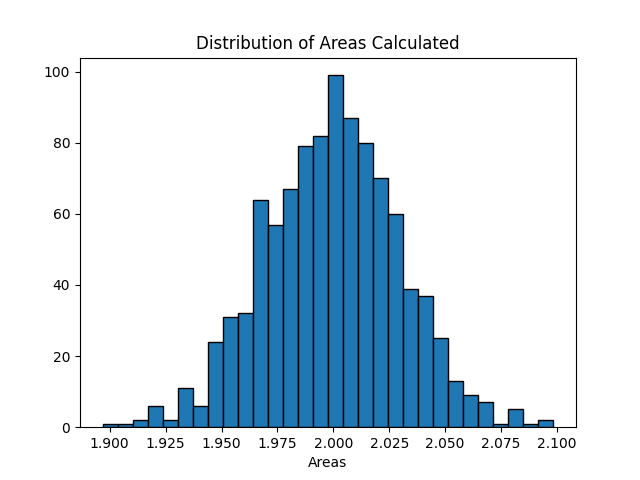
\includegraphics[width=0.75\linewidth]{montecarlo.png}
    \caption{1st histogram showing seemingly random distribution of approximations of Area using M-C (Monte Carlo)}
\end{figure}
    \begin{figure}
        \centering
        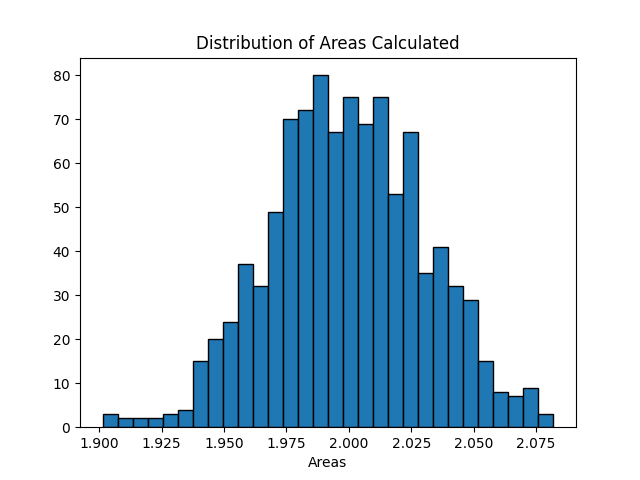
\includegraphics[width=0.75\linewidth]{montecarlo2.png}
        \caption{2nd histogram, same depiction as Figure 1}
        \label{fig:enter-label}
    \end{figure}
    \begin{figure}
        \centering
        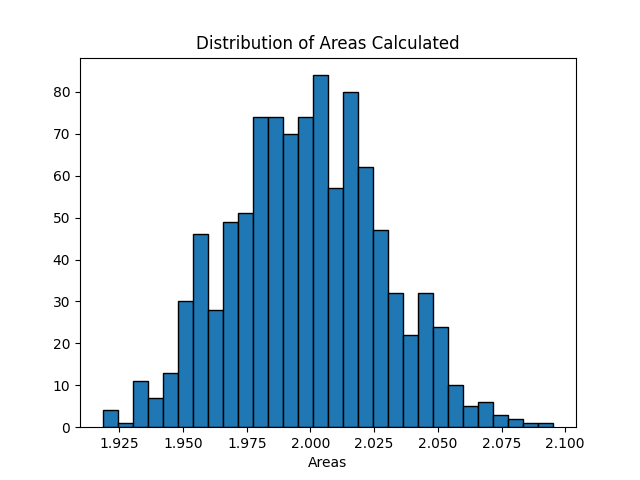
\includegraphics[width=0.75\linewidth]{montecarlo3.png}
        \caption{3rd Histogram, same depiction as Figure 1 and 2}
        \label{fig:enter-label}
    \end{figure}
    \label{}
\section{Conclusion on data}
It is clear that as n tends to infinity, and gets larger, we would see that the frequency of the bars closest to and containing an area of 2.000, would increase, and the distribution would form close to a specific Dirac Distribution. The code is in my GitHub, and if you wish to experiment and visualise what would happen as n increases, you can take and edit the code, and see for yourself how it affects the distribution. I also have the code for the Monte Carlo Integration itself, as this is what the paper mainly outlines. Thank you for reading this.

\section{Links and connections}
GitHub: CauchyIntegrah (Adam A.)

\end{document}
